\section{Gesichtserkennung} \label{sec:recognition}
\begin{tcolorbox}
	\centerline{\textbf{Lernziele Kapitel~\ref{sec:recognition}}}
	\begin{enumerate}[leftmargin=*,label=\thesection.\arabic*]
		\item \label{item:recognition} Die Lernenden können erklären, wie die Eigengesichter das \glqq{}ähnlich aussehen\grqq{} von Gesichtern quantifizieren können.\\
		(Aufgaben~\ref{aufg:quantification} und~\ref{aufg:quantification_code})
	\end{enumerate}
\end{tcolorbox}
Nun wollen wir die Eigengesichter nutzen für eine Gesichtserkennung nutzen.
Wie bereits in der Einleitung erklärt, ist Gesichtserkennung im Grunde eine Klassifizierung.
Hier als Beispiel betrachten wir 8 verschiedene Klassen.
\begin{table}[ht]
	\centering
	\begin{tabular}{|c|c|c|c|}
		\hline
		Daniel Radcliffe & Emma Stone & Emma Watson & Eva Green \\
		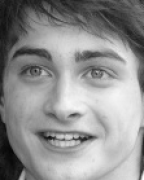
\includegraphics[width=0.2\textwidth]{images/recognition/Daniel_Radcliffe} & 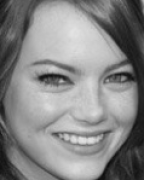
\includegraphics[width=0.2\textwidth]{images/recognition/Emma_Stone} & 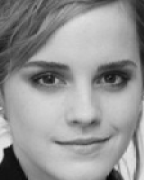
\includegraphics[width=0.2\textwidth]{images/recognition/Emma_Watson} & 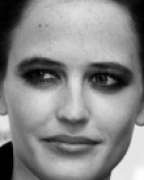
\includegraphics[width=0.2\textwidth]{images/recognition/Eva_Green} \\ \hline
		Jennifer Lawrence & Orlando Bloom & Pierce Brosnan & Tom Cruise \\
		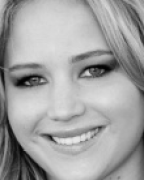
\includegraphics[width=0.2\textwidth]{images/recognition/Jennifer_Lawrence} & 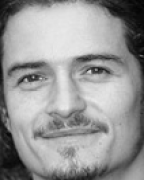
\includegraphics[width=0.2\textwidth]{images/recognition/Orlando_Bloom} & 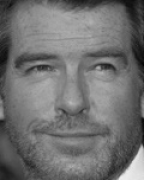
\includegraphics[width=0.2\textwidth]{images/recognition/Pierce_Brosnan} & 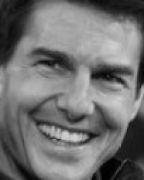
\includegraphics[width=0.2\textwidth]{images/recognition/Tom_Cruise} \\ \hline
	\end{tabular}
	\caption{Die acht verschiedenen Klassen. }
	\label{tab:classes}
\end{table}
Wir verwenden in diesem Kapitel eine Datenbank die nur aus Bilder dieser 8 Personen besteht.
Dabei enthält sie von jeder Person genau 10 Bilder.
Das heisst, sie besteht aus $K=8\cdot 10=80$ Bildern.
Pro Klasse haben wir zusätzlich 3 Testbilder.
Das sind Bilder die zwar jeweils eine dieser 8 Personen zeigen, aber nicht in der Datenbank enthalten sind.
Das Ziel ist nun die Testbilder möglichst der richtigen Klasse zuzuordnen.
So können wir unsere Gesichtserkennung testen, daher der Name \glqq{}Testbilder\grqq{}.
\begin{figure}[ht]
	\centering
	\begin{tabular}{|c m{2cm} m{2cm} m{2cm} m{2cm} m{2cm}|}
		\hline
		Datanbank &
		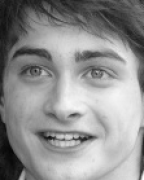
\includegraphics[width=0.1\textwidth]{images/recognition/training_faces/training_0} &
		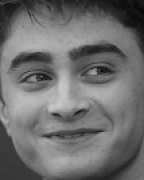
\includegraphics[width=0.1\textwidth]{images/recognition/training_faces/training_1} &
		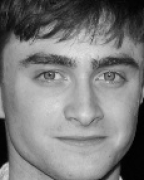
\includegraphics[width=0.1\textwidth]{images/recognition/training_faces/training_2} &
		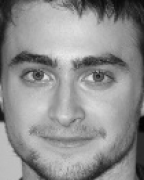
\includegraphics[width=0.1\textwidth]{images/recognition/training_faces/training_3} &
		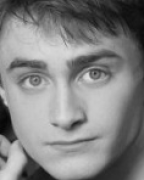
\includegraphics[width=0.1\textwidth]{images/recognition/training_faces/training_4} \\
		&
		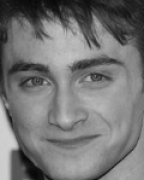
\includegraphics[width=0.1\textwidth]{images/recognition/training_faces/training_5} &
		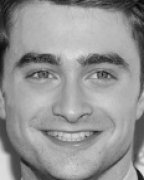
\includegraphics[width=0.1\textwidth]{images/recognition/training_faces/training_6} &
		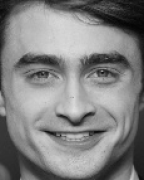
\includegraphics[width=0.1\textwidth]{images/recognition/training_faces/training_7} &
		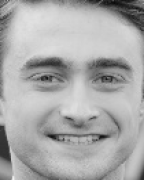
\includegraphics[width=0.1\textwidth]{images/recognition/training_faces/training_8} &
		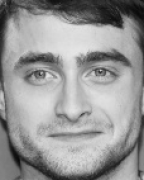
\includegraphics[width=0.1\textwidth]{images/recognition/training_faces/training_9} \\ \hline
		Testbilder &
		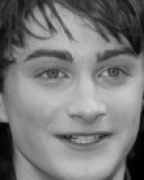
\includegraphics[width=0.1\textwidth]{images/recognition/test_faces/test_0} &
		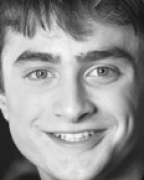
\includegraphics[width=0.1\textwidth]{images/recognition/test_faces/test_1} &
		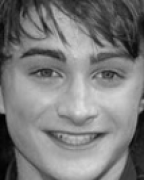
\includegraphics[width=0.1\textwidth]{images/recognition/test_faces/test_2} &
		& \\ \hline
	\end{tabular}
	\caption{Datenbank- und Testbilder am Beispiel der Klasse \glqq{}Daniel Radcliffe\grqq{}}
	\label{fig:testfaces}
\end{figure}
Zwar ist das für einen Menschen ganz leicht, aber für einen Computer ist das überhaupt nicht einfach.
Im Grunde müssen wir den Computer lehren, wann zwei Bilder ähnlich aussehen.
Dazu brauchen wir ein Mass für die Distanz zweier Bilder.
Es stellt sich heraus, dass die Eigengesichter ein Solches liefern.
Seien nun $\vec p$ und $\vec q$ zwei Bilder von Gesichtern.
Wir schreiben die entsprechenden Differenzgesichter als Linearkombination der Eigengesichter
\begin{equation*}
	\vec p-\vec m=c_1\vec u_1+c_2\vec u_2+\ldots+c_K\vec u_K
\end{equation*}
und
\begin{equation*}
	\vec q-\vec m=\tilde c_1\vec u_1+\tilde c_2\vec u_2+\ldots+\tilde c_K\vec u_K,
\end{equation*}
wobei nun $K=80$ und $\vec m$ das Durchschnittsgesicht der Bilder der neuen Datenbank ist.
Entsprechend sehen die Eigengesichter auch etwas anders aus, aber deren Eigenschaften sind die selben.
Das besagte Mass der Distanz zwischen den Gesichtern $\vec p$ und $\vec q$ definieren wir als
\begin{equation*}
	D\left(\vec p,\vec q\right)=\left(c_1-\tilde c_1\right)^2+\left(c_2-\tilde c_2\right)^2+\ldots+\left(c_K-\tilde c_K\right)^2.
\end{equation*}
\begin{aufgabe} \label{aufg:quantification}
	Warum entspricht dieser Begriff von Distanz dem \glqq{}Ähnlich aussehen\grqq{} von Gesichtern?
	Erklären Sie in Worten.
	\textit{Hinweis:} Rufen Sie sich die Konstruktion der Eigengesichter und die Diskussion am Ende von Kapitel~\ref{sec:facespace} in Erinnerung.
\end{aufgabe}
\begin{losung}
	Die Eigengesichter fangen gewisse Gesichtszüge ein.
	Die Funktion $D\left(\vec p,\vec q\right)$ vergleicht, wie fest sich $\vec p$ und $\vec q$ in eben diesen Gesichtszügen unterscheiden.
	Dabei werden die ersten Eigengesichter am stärksten gewichtet, da ihre Koeffizienten typischerweise am grössten sind (Abbildung~\ref{fig:coef}).
	Das macht auch Sinn, denn es sind genau die ersten Eigengesichter (Gesichtszüge), in denen sich die Gesichter der Datenbank am meisten unterscheiden.
	Die Bilder nur Pixel für Pixel zu vergleichen macht keinen Sinn, denn kein Pixel kann alleine eine Information über ein Gesicht tragen.
	Anders gesagt können sich zwei Bilder in jedem Pixel stark unterscheiden und dennoch die selbe Person zeigen.
	Mit Gesichtszügen ist dies kaum möglich.
\end{losung}
Sei nun ein Bild $\vec p$ gegeben, das nicht notwendigerweise in der Datenbank enthalten ist.
Das Bild soll zudem eine der 8 Personen aus Tabelle~\ref{tab:classes} zeigen.
Jedoch wissen wir nicht welche.
Wir werden versuchen das mit folgendem Verfahren zu erraten.
\begin{enumerate}[leftmargin=3cm, label=Schritt \arabic*:]
	\item Seien $\vec q_1,\ldots,\vec q_{80}$ die Bilder der Datenbank.
	Wir berechnen die Distanz $D\left(\vec p,\vec q_i\right)$ für $i=1,\ldots,80$.
	\item Eines dieser Bilder wird die kleinste Distanz zu $\vec p$ haben, sagen wir das ist $\vec q_j$ für ein bestimmtes $1\leq j\leq 80$.
	\item Wir schauen in der Datenbank nach, welche Person auf dem Bild $\vec q_j$ gezeigt ist. Da $\vec p$ ähnlich aussieht, zeigt es wohl die selbe Person und wir klassifizieren $\vec p$ entsprechend.
\end{enumerate}
\begin{aufgabe} \label{aufg:quantification_code}
	Ergänzen sie die Funktion \texttt{distance(p, q, m, u\_list)} welche die Distanz $D\left(\vec p,\vec q\right)$ zweier Bilder zurück gibt.
	Dabei ist \texttt{m} das Durchschnittsgesicht und \texttt{u\_list} enthält die Liste der Eigengesichter.
	Die Variablen \texttt{p} und \texttt{q} enthalten die Vektoren $\vec p$ und $\vec q$.
	Testen Sie ihre Implementation indem Sie das Skript \texttt{recognition.py} ausführen.
	\textit{Hinweis:} Verwenden sie die Funktion \texttt{compute\_coefficients(...)} aus Aufgabe~\ref{aufg:compute_coefficients}.
\end{aufgabe}
\begin{losung}
	Die Lösung könnte zum Beispiel so aussehen.
\begin{lstlisting}[style=python]
def distance(p, q, m, u_list):
	cp = compute_coefficients(p, m, u_list)
	cq = compute_coefficients(q, m, u_list)
	d = (cp - cq)
	return np.dot(d, d)
\end{lstlisting}
Der Output von \texttt{recognition.py} ist in Tabelle~\ref{tab:recognition} gelistet.
\end{losung}
\begin{table}[ht]
	\centering
	\begin{tabular}{|l|c|c|}
		\hline
		\textbf{Klasse} & \textbf{Anzahl Testbilder} & \textbf{davon richtig klassifiziert} \\ \hline
		Daniel Radcliffe & 3 & 1 \\ \hline
		Emma Stone & 3 & 3 \\ \hline
		Emma Watson & 3 & 1 \\ \hline
		Eva Green & 3 & 2 \\ \hline
		Jennifer Lawrence & 3 & 3 \\ \hline
		Orlando Bloom & 3 & 1 \\ \hline
		Pierce Brosnan & 3 & 1 \\ \hline
		Tom Cruise & 3 & 2 \\ \hline
	\end{tabular}
	\caption{Resultate der Gesichtserkennung.}
	\label{tab:recognition}
\end{table}
Aus Tabelle~\ref{tab:recognition} ist zu entnehmen, dass von den insgesamt $3\cdot8=24$ Testbildern $14$ richtig klassifiziert wurden.
Dies entspricht einer Erfolgsquote von $\frac{14}{24}=0.58333\ldots$, also knapp $60\%$.
Zum Vergleich: Würde man die Testbilder einfach zufällig den Klassen zuordnen, so wäre die erwartete Erfolgsquote $\frac{1}{8}=0.125$, also $12.5\%$.